\documentclass[11pt]{article}
\usepackage{colacl}
\usepackage{appendix}
\usepackage{graphicx}
\renewcommand{\appendixpagename}{\Large Appendices} %	10pt
\usepackage{listings}
\sloppy



\title{HPC Twitter GeoProcessing Report}
\author
{Zichun Zhu, Xiaoyue Ma}

\begin{document}
\maketitle


\section{Introduction}

\section{Methodology}

\subsection{HPC Parallelism}
In general there are two approaches to parallelize a program: divide work by data, and divide work by steps. The chosen is highly depend on the specification of work. In geo processing, the number of steps per data entity is relatively small, while the size of whole data could be very large. Thus dividing work by data, and assigning working on a piece of data to different processes is more tractable.

\subsection{MPI}
There are different ways to classifiy parallel computers. The widely used classification, Flynn's taxonomy distinguishes computer architecture along instruction stream and data stream. According its definition, most current High Performance Computer(HPC) is in Multiple Instruction, Multiple Data(MIMD) type. Every process can work concurrently on different data stream, but those data and processors could be physically located in different place. To share the data between the processors,  we applied MPI in the implementation.

Message Passing  Interface(MPI) is an useful open source tool in multi-core programming which contains many functions to share message in processes. The main difference between OpenMP and MPI is that the processes using MPI does not shared memory between each other, while OpenMP is a shared memory multiprocessing programming library.  MPI therefore able to be used in wide application regardless the physical architecture of platform.

Considering that the size of data could be up to 15 GB, even though divided into chunks it is still a heavy load message transmission. So rather than reading the whole data and then sending out pieces of raw data, the master process scans and records the line indexes, and then scatters the indexes instead. A simple calculation can imply the efficiency and sufficiency. In $smallTwitter.json$, there are 
about 7000 lines, each is one tweet, and the size of the file is about 25 MB. If we assume tweets density is even, a 15 GB file may contains: \[tweet\_num = 25MB / 15GB * 7000 \approx 4.2million\] If those tweets are represented in indexes, and each takes size of $int$, then 15 GB tweets file can be abstracted to: \[indexes\_size = 4.2million * 24bytes \approx 100MB \] The load of transmission could be largely reduced by representing tweets in form of indexes. 



\section{Result}

\begin{table}[]
\begin{tabular}{c|ccc}
\multicolumn{1}{l|}{Speedup(s)} & \multicolumn{1}{l}{Real} & \multicolumn{1}{l}{User} & \multicolumn{1}{l}{Sys} \\ \hline
1 Node 1 Task                   & 342.685                  & 328.387                  & 12.025                  \\ \hline
1 Node 8 Task                   & 122.154                  & 961.023                  & 13.059                  \\ \hline
2 Node 8 Task                   & 140.352                  & 376.636                  & 181.978                
\end{tabular}
\caption{Runtime}
\label{Runtime}
\end{table}

\begin{table}[]
\begin{tabular}{c|c}
\multicolumn{1}{l|}{Runtime(s)} & \multicolumn{1}{l}{Speed up} \\ \hline
1 Node 1 Task                   & 1                            \\
1 Node 8 Task                   & 2.81                         \\
2 Node 8 Task                   & 2.44                        
\end{tabular}
\caption{Speedup}
\label{Speedup}
\end{table}
\begin{figure}[h]
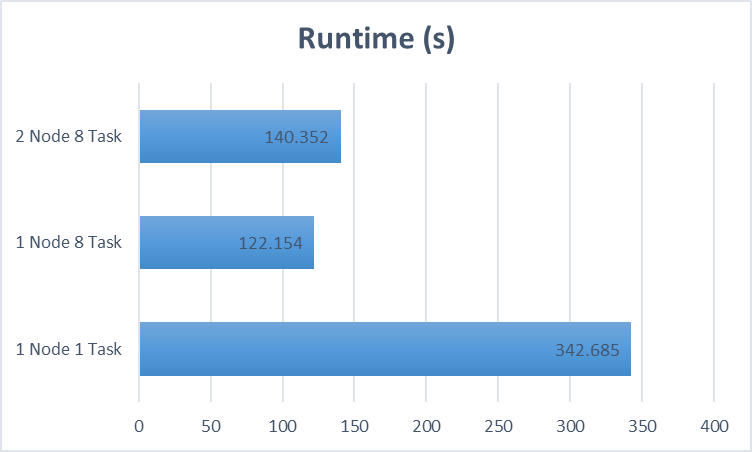
\includegraphics[width=0.8\textwidth]{Runtime}
\end{figure}

\begin{appendices}
\appendixpage
\section{Slurm Script}
\subsection{1 Node 1 Task}
\lstinputlisting[language=sh]{1node1task.slurm}
\subsection{1 Node 8 Task}
\lstinputlisting[language=sh]{1node8task.slurm}
\subsection{2 Node 8 Task}
\lstinputlisting[language=sh]{2node8task.slurm}
\end{appendices}

\end{document}
